\section{Transmon source\label{sec:transmon}}

It has experimental  coherence times of $ \sim 100\,\mu  $s.  The Transmon
paper  by Sam  Bader  December  2013. There  are  two  main factors  to
consider when making a Cooper pair box
\begin{equation}\label{key}
  \mathcal{H} = E_C{\left(\hat{\red{N}}-N_\text{ext}\right)^2}- E_J\cos\left(\hat{\blue{\phi}}\right),
\end{equation}
\noindent which was discussed in Ch.~\ref{sec:cooper_pair_box}.

\begin{itemize}
\item    $   \mathbf{E_C/E_J    >>    1    }$   {High    anharmonicity,
    $  \frac{E_{12} -  E_{01}}{E_{01}}\approx -(8E_J/E_C)^{-1/2}  $, allowing
    addressation of individual transitions};
\item $ \mathbf{E_C/E_J  <<1 }$ {Low charge noise  sensitivity, so that
    $  N_\text{ext} $  does not  jump and  affect the  quadratic energy
    dependance};
\end{itemize}

\noindent    \red{\textbf{It     is    usually    better     to    have
    $ \mathbf{E_C/E_J  <<1 }$, because anharmonicity  decreases slowly,
    while the charge sensitivity will greatly improve.}} To do this, we
need to increase the apparent capacitance  of the junction with a large
shunt capacitance:

\begin{figure}[h]
  \centering 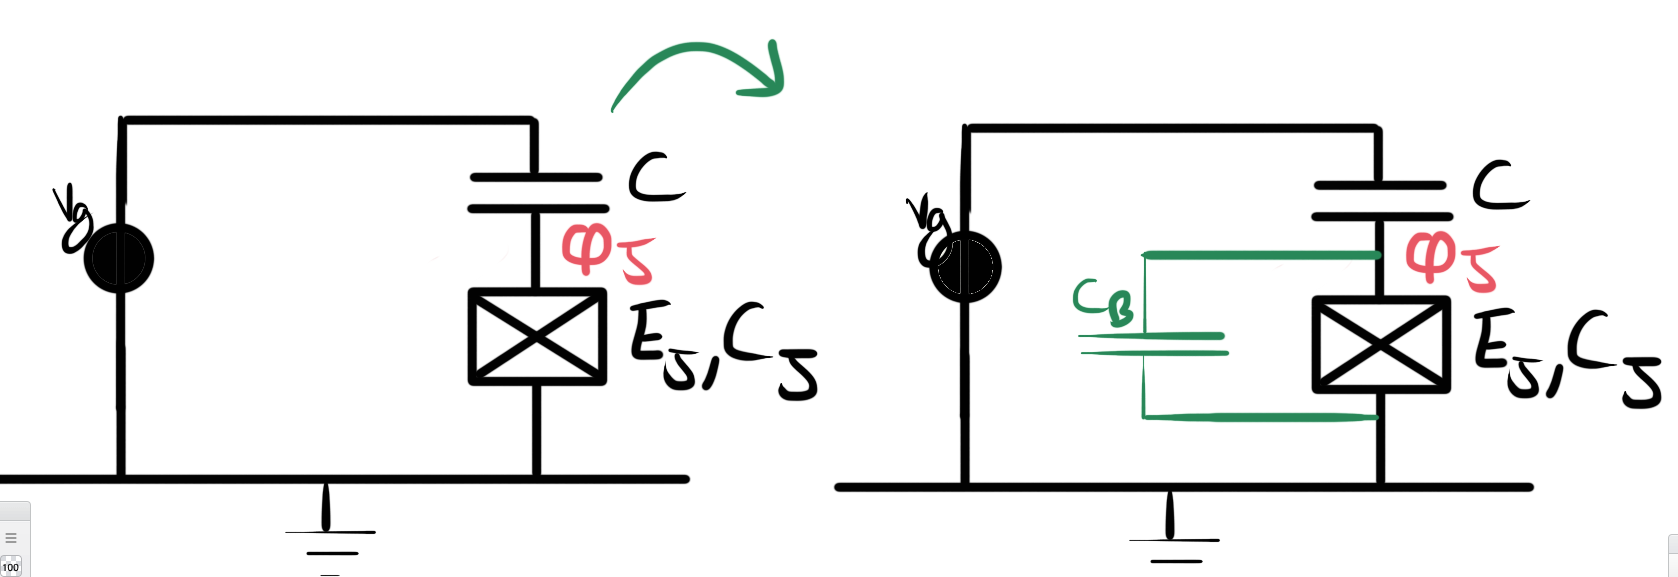
\includegraphics[height=4cm]{transmon_1}
\end{figure}

\noindent

\begin{framed}\noindent
  The same  equations are used as  for the Cooper pair  box, except the
  capacitance $ C_J \rightarrow C_B$, which is magnitudes larger.
  \begin{equation}\label{key}
    \mathcal{H}_\text{transmon} = E_C{\left(\hat{\red{N}}-N_\text{ext}\right)^2}- E_J\cos\left(\hat{\blue{\phi}}\right),
  \end{equation}

\end{framed}

\newpage
